\documentclass[10pt,a4paper]{report}
\usepackage[utf8]{inputenc}
\usepackage[spanish]{babel}
\usepackage{amsmath}
\usepackage{amsfonts}
\usepackage{amssymb}
\usepackage{steinmetz}
\usepackage{circuitikz}
\usepackage{halloweenmath}
\usepackage[normalem]{ulem}
%\usepackage{steinmetz}
%\usepackage[american,siunitx]{circuitikz}
\usetikzlibrary{arrows,shapes,shapes.geometric, arrows.meta,calc,positioning,babel}
\usetikzlibrary{backgrounds}
\usetikzlibrary{fit}
%\usetikzlibrary{shapes.geometric, arrows.meta, positioning, calc}
%%%%%%%%%%%%%%%%%%%%%%%%%%%%%%%%%%%%%%%%%%%%%%%%
\usepackage{listings}
\usepackage{xcolor}

\definecolor{codegreen}{rgb}{0,0.6,0}
\definecolor{codegray}{rgb}{0.5,0.5,0.5}
\definecolor{codepurple}{rgb}{0.58,0,0.82}
\definecolor{backcolour}{rgb}{0.95,0.95,0.92}

\lstdefinestyle{mystyle}{
	backgroundcolor=\color{backcolour},   
	commentstyle=\color{codegreen},
	keywordstyle=\color{magenta},
	numberstyle=\tiny\color{codegray},
	stringstyle=\color{codepurple},
	basicstyle=\ttfamily\footnotesize,
	breakatwhitespace=false,         
	breaklines=true,                 
	captionpos=b,                    
	keepspaces=true,                 
	numbers=left,                    
	numbersep=5pt,                  
	showspaces=false,                
	showstringspaces=false,
	showtabs=false,                  
	tabsize=2
}
\lstset{style=mystyle}
%%%%%%%%%%%%%%%%%%%%%%%%%%%%%%%%%%%%%%%%%%%%%%%%
\usepackage{graphicx}
\usepackage{multirow}
\usepackage[hyperindex=true,breaklinks=true,colorlinks=true,linkcolor=blue]{hyperref}
\usepackage{multimedia}
\usepackage{subfig}
\usepackage{dirtree}
\addto\captionsspanish{
\renewcommand{\tablename}{Tabla}
\renewcommand{\listtablename}{\'Indice de Tablas}
\addto\captionsspanish{
  \renewcommand{\lstlistingname}{Listado}
  \renewcommand{\lstlistlistingname}{\'Indice de listados}
}
}

\usepackage{makeidx}
\usepackage[left=2cm,right=2cm,top=2cm,bottom=2cm]{geometry}
\title{

\includegraphics[scale=0.15]{ucm2.eps} Universidad Complutense de Madrid\\
------------------------------------------------------------------------------------\\
Documentación del software desarrollado para la práctica de control de un motor de cc}
\author{Juan Jiménez}
\graphicspath{{./FIGURAS/}}
\newcommand{\mymotor}[2] % #1 = name , #2 = rotation angle
{\draw[thick,rotate=#2] (#1) circle (10pt)
 node[]{$\mathsf M$} 
++(-12pt,3pt)--++(0,-6pt) --++(2.5pt,0) ++(-2.8pt,6pt)-- ++(2.5pt,0pt);
\draw[thick,rotate=#2] (#1) ++(12pt,3pt)--++(0,-6pt) --++(-2.5pt,0) ++(2.8pt,6pt)-- ++(-2.5pt,0pt);
}

\newcommand{\mymotorB}[2] % #1 = name 
{\draw[thick] (#1) circle (12pt)
node[above=-3pt]{$\mathsf M$} ++(-8pt,-3pt)--++(15pt,0);
\draw[thick,dashed] (#1) ++(-8pt,-5pt)--++(15pt,0);
}

\makeindex
\begin{document}
\maketitle
\vspace*{\fill}

\includegraphics[scale=1]{by-sa.eps}\\
El contenido de estos apuntes est\'a bajo licencia Creative Commons Atribution-ShareAlike 4.0\\
\href{http://creativecommons.org/licenses/by-sa/4.0/}{http://creativecommons.org/licenses/by-sa/4.0/}\\
\copyright Juan Jim\'enez

\bigskip
\tableofcontents
\listoffigures
\listoftables
\abstract{Estas notas son complementarias al guión de la práctica y explican todo el proceso de construcción del software empleado el la práctica. Dan información de los IDEs empleados para el desarrollo del software, de su instalación, de la configuración de la placa de control empleada y de la estructura de los programas desarrollados}
% !TEX root = making_of.tex
\chapter{Primeros pasos}
\section{Sofware necesario}
En primer lugar, como se ha explicado ya en el guión de la práctica, vamos a emplear la placa STM32F411E, de la compañía ST, para controlar el motor. En la jerga de los programadores de microcontroladores, esta placa es conocida como la \emph{Black Pill}. Una de sus ventajas, es que tiene un excelente soporte de sofware y herramientas de desarrollo.

En esta sección vamos a describir como a asumir que estamos trabajando con un ordenador personal con sistema operativo Linux, en concreto vamos a emplear Ubuntu 24.04.4 LTS.
	\begin{verbatim}
	https://ubuntu.com/download/desktop
	\end{verbatim}


Algunas herramientas básicas necesarias son:
\begin{enumerate}
	\item Visual studio Code (VSC).	
Será el entorno de desarrollo que emplearemos para escribir, compilar y descargar el código que utilizará la placa ST. También servirá para desarrollar el código en Python que nos permitirá comunicarnos y controlar la placa desde el ordenador. Para instalarlo en Ubuntu, lo ideal es descargar directamente el paquete .dev, de la página web de VSC,
\begin{verbatim}
	https://code.visualstudio.com/thank-you?dv=linux64_deb
\end{verbatim}
para instalarlo ir a la línea de comandos:
\begin{verbatim}
sudo apt install ./Descargas/code_*.deb	
\end{verbatim}

Ver descripción detallada en el capítulo \ref{capvs}
	
	\item STM32CubeMX: Es la herramienta gráfica oficial de ST. Sirve para 	configurar los pines, el reloj (clock) y generar el código base en C.
	\begin{verbatim}
	https://www.st.com/en/development-tools/stm32cubemx.html
	\end{verbatim}

	\item STM32CubeCLT:
	Tiene todas las herramientas de ST, necesarias para compilar, enlazar etc.
	Para instalarlo
	Descargar de la página web de ST,
	\begin{verbatim}
	https://www.st.com/en/development-tools/stm32cubeclt.html
	\end{verbatim}
	el que pone Debian Linux installer.
	Descomprimir,
	\begin{verbatim}
		unzip st-stm32cubeclt_1.21.0_27995_20260219_1804_amd64.deb_bundle.sh.zip
	\end{verbatim}
	Dar Permisos
	\begin{verbatim}
		chmod +x st-stm32cubeclt_1.21.0_27995_20260219_1804_amd64.deb_bundle.sh
	\end{verbatim}
Lanzar el instalador
\begin{verbatim}
sudo ./st-stm32cubeclt_1.21.0_27995_20260219_1804_amd64.deb_bundle.sh	
\end{verbatim}
Presentará en el terminal la licencia de uso, ir hasta el final y aceptarla.
Debería instalarlo en:
\begin{verbatim}
	/opt/st/stm32cubeclt_1.21.0/
\end{verbatim}
Es toolset STM32CubeCLT incluye:

\begin{itemize}
	\item GNU C/C++ for Arm® toolchain tales como arm-none-abi-gcc(compilador), arm-none-abi-nm (symbol viewer) y otros.
	\item GDB debugger cliente y servidor (Depurador). Depurar el programa ejecutándolo en la propia placa
	\item STM32CubeProgrammer (STM32CubeProg) utility (Programador) Descargar el ejecutable desde el ordenador a la placa.
	\item System view descriptor files (.SVD) for the entire STM32 MCU portfolio.
    \item Map file associating STM32 MCUs and MCU development boards to the appropriate SVD 
\end{itemize}

	\item Cmake y Ninja: fundamentales para gestionar la construcción del proyecto: Librerías, dependencias, etc.
	
	\item ST-Link Drivers: permite la comunicación entre el ordenador y la placa de desarrollo a través de un puertos USB. Estas dos últimas herramientas se instalan directamente desde VSC. (Ver capitulo \ref{capvs})
	\item Python y los modulos de Python: serial, struct, csv, sys, time, collections, datetime, pyqtgraph.
	\item (Opcional) Si se va a hacer el análisis de los datos y los modelos del motor en python, entonces es comveniente instalar también los módulos: pandas, numpy, matplotlib.pyplot y control
	
Para instalar STM32CubeMx, lo ideal es obtenerlo de la página web de ST,

\noindent https://www.st.com/en/development-tools/stm32cubemx.html

Igualmente, para STM32CubeProgrammer,

\noindent
https://www.st.com/en/development-tools/stm32cubeprog.html

El resto de las herramientas, se pueden instalar directamente a través de Visualstudio Code, Mediante las extensiones para SMT32.

En el caso de Python, es bastante cómodo instalar directamente anaconda.

https://www.anaconda.com/downloadP

Varios de los módulos de Python necesarios vienen instalados por defecto con Anaconda y el resto son fácilmente instalables empleando \texttt{conda}.
 
\end{enumerate}

% !TEX root = making_of.tex
\chapter{El entorno de desarrollo de Visual Studio Code (VSC)}\label{capvs}
Entre las diferentes opciones existentes de IDEs (Integrated development Environments), se ha optado por emplear el programa Visual Studio Codepara el desarollo de este proyecto.

\begin{figure}
	
\includegraphics[width=\textwidth]{vsscreen.png}
	\caption{Ventana de Visual Studio Code} \label{fig:vscr}
\end{figure}

Si abrimos el programa, una vez instalado, accedemos a una ventana como la se muestra en la figura \ref{fig:vscr}. Vamos a describir brevemente los elementos más importantes.

\begin{itemize}
	\item Barra de actividad: Es la barra vertical localizada a la izquierda del todo de la ventana. Esta barra permite cambiar la vista del panel situado inmediatamente a su derecha. Las distinta opciones hacen referencias a tareas distintas realizables desde VSC. Así el icono superior (Explorer nos permite navegar por los directorios que tenemos abierto, seleccionar archivos para abrirlos en el editor etc. Debajo tenemos una opción de búsqueda (Search). Un control de cambios basado en git (Source control). Un botón para ejecución y depuración de código (RUN and debug), Un botón muy útil que nos permite explorar las extensiones (Extensions) disponibles, es decir configuraciones específicas para manejar distintos tipos de lenguajes de programación, etc.
	\item Barra Lateral, inmediatamente a la derecha de la anterior, ofrece distintas vistas y paneles, dependiendo de la actividad seleccionada en la barra de actividad. En la figura \ref{fig:vscr}, se ve el panel correspondiente a las extensiones, porque la actividad seleccionada, ha sido precisamente el botón extensions. Se pueden recorrer las extensiones disponibles, comprobar si están o no instaladas, y seleccionarla para su instalación/desinstalación, configuración, etc.
	\item El editor. Ocupa el area central. Su objetivo es escribir y editar código. Es posible abrir varios editores uno al lado del otro y de este modo trabajar en varios archivos simultáneamente. En la figura \ref{fig:vscr}, se muestra un fichero de texto que contiene la fuente el \LaTeX con la que se han elaborado estas notas. A su derecha, se ve el texto resultante en un archivo pdf.
	\item Barra de estado (Status Bar) Situada en la parte inferior de la ventana, ofrece información contextual relacionada con el estado actual de VSC y la actividad que se está llevando a cabo.
	\item Paleta de Comandos (Command Palette) Se accede pulsando los comandos Ctrl + Shift + P, es muy útil porque permite el acceso rápido a muchos comandos y características de VSC, sin tener que navegar por menús de opciones.
	\item Paneles. Estań localizados debajo del editor. Muestran distintas herramienta muy útiles. Terminales del sistema, Salidas para los distintos compiladores, Consolas de depuración, panel de problemas etc.
	\item Tabs. Situados en la parte superior del editor, permiten intercambiar la vista entre los archivos abiertos.  
\end{itemize}

Una vez instalado VSC debemos seleccionar las extensiones adecuadas para poder compilar codigo C, para la placa, descargarlo y, en su caso, poder depurarlo.

Además, podemos también instalar las extensiones para escribir y ejecutar código en python. De esta manera, con un solo IDE, podemos generar todo el código necesario; tanto el código en C para la placa controladora como en código en Python para interactuar con al placa desde el ordenador.

\section{Instalación de las extensiones STM32Cube}
Tanto para el desarrollo de código C para la placa STM32F411E como para compilar dicho código y descargarlo en la placa, necesitamos instalar las extensiones necesarias de STM32Cube.

Para hacerlo, pulsamos en la barra de actividades, el botón de las extensiones que tiene un icono con cuatro cuadros. Automaticamente aparecerá en la barra lateral las extensiones disponibles. Lo más sencillo es escribir en la barra de búsqueda la extensión que deseamos instalar: \texttt{STM32CubeIDE for Visual Studio Code}. Las extensiones de ST, empelan como símbolo una mariposa sobre un círculo azul, seleccionamos la que hemos buscado, pulsamos en el botón 'install'. Dejamos que complete la instalación. Estamos ya en condiciones de escribir, compilar y descargar código para nuestra placa ST.

\section{Instalación de las extensiones para Python}
VSC, puede emplear directamente la instalación de Python existente en nuestro ordenador. Sin embargo, como ya hemos indicado, es particularmnente cómodo manejarlo desde la distribución de anaconda.

Para poder manejar python desde VSC podemos emplear la extensión 'Pylance' El procedimiento de instalación es idéntico al que hemos visto para Las extensiones de ST. Buscamos Pylance en el buscador de las extensiónes y pulsamos el botón 'Install'.

Una vez instalado, VSC reconocerá cualquier archivo con extensión .py como propio de Python y nos mostrará a, la altura de los tabs, un triángulo verde. Si lo pulsamos ejecutará, en el terminal, disponible en los paneles, el código de archivo .py abierto en el editor activo.

Es posible que en la primera ejecución nos pregunte que interprete de python queremos emplear, seleccionar el señalado como 'conda', asociado a la distribución de Anaconda.
% !TEX root = making_of.tex
\chapter{Configuración de la placa con STM32CubeMX}
STM32CubeMx, es una herramienta extremadamente útil para configurar el Hardware de nuestra placa. Conocer a fondo todas sus posibilidades está fuera de los objetivos de estas notas. Aquí nos vamos a centrar en configurar la placa para que pueda controlar nuestro motor. Lo vamos ha hacer paso a paso.

Al ejecutara STMCube32MX, se abre una primera ventana e la que se nos permite abrir proyectos ya existentes o crear proyectos nuevos figura (\ref{fig:stmx}). Entre las opciones para crear proyectos nuevos, podemos emplear tanto el botón \texttt{ACCESS TO MCU SELECTOR} como el botón \texttt{ACCESS TO BOARD SELECTOR}. La diferencia es que en el primer caso nos selecciona el microcontrolador, y no nos configura nada por defecto. Si seleccionamos la placa el Package pgfkeys Error: I do not know the key '/tikz/fit', to which you passed '(tim4) (update) (cnt) (txdma)', and I am going to ignore it. Perhaps you misspelled it.programa sabe qué pines están conectados al led y al botón azul de usuario y además configura la emulación del puerto serie, a través del puerto USB de la placa, para comunicar la placa con el ordenador. Si empleamos la primera opción, tendremos que configurar nosotros a mano estas opciones, caso de que queramos usarlas.

Vamos a seleccionar directamente la placa núcleo que la que vamos a trabajar. Para ello pulsamos el botón \texttt{ACCESS TO BOARD SELECTOR}. Se abrirá una nueva ventana, figura (\ref{fig:cdiagram}). Seleccionamos en la entrada \texttt{comercial part number}, arriba a la izquierda, nuestra placa: NUCLEO F411RE. Esperamos a que la seleccione y nos abrirá una pequeña ventana de diálogo en la que nos sugiere inicializar todos los periféricos con las opciones por defecto.Seleccionamos \texttt{no}. Se cierra la ventana de selección y en la ventana principal de STM32CubeMX aparecen varias pestañas y se nos muestra el pinout de la placa con los pines que ya están configurados por defecto, el color y 'fijados' con una chincheta figura (\ref{fig:layoutp}).

\section{Placa en modo debug y reseteo del pin PB3}
Lo primero que vamos ha hacer, es poner la placa en modo debug. Hacemos esto para que nos deje programar la placa siempre que queramos sin necesidad de emplear el botón de reset. Para ello, desplegamos el menú \texttt{System Core}, seleccionamos la opcion \texttt{SYS} y se nos abrirá un panel de configuración, figura (\ref{fig:PB3}). En la entrada que pode \texttt{Debug}, seleccionamos \texttt{Serial Wire}. A continuación vamos a liberar el pin \texttt{B3}. Por defecto este pin está configurado precisamente para emplear el método de depuración \texttt{Serial Wire} y aparece marcado con las letras \texttt{SWO} (Serial Wire Output). Pero nosotros no necesitamos emplear ese modo de depuración y lo que vamos ha hacer es resetearlo para poder emplearlo como pin de control del movimiento del motor (ver tabla \ref{tab:pines}) más alante. Para resetearlo lo seleccionamos con el ratón el esquema mostrado en el panel \emph{pinout view} y en el menú desplegable que aparece seleccionamos \texttt{Reset\_State} El pin se pondrá de color gris.

\begin{figure}

\centering
\subfloat[Ventana inicial de STMCube32MX]{\label{fig:stmx}
\centering
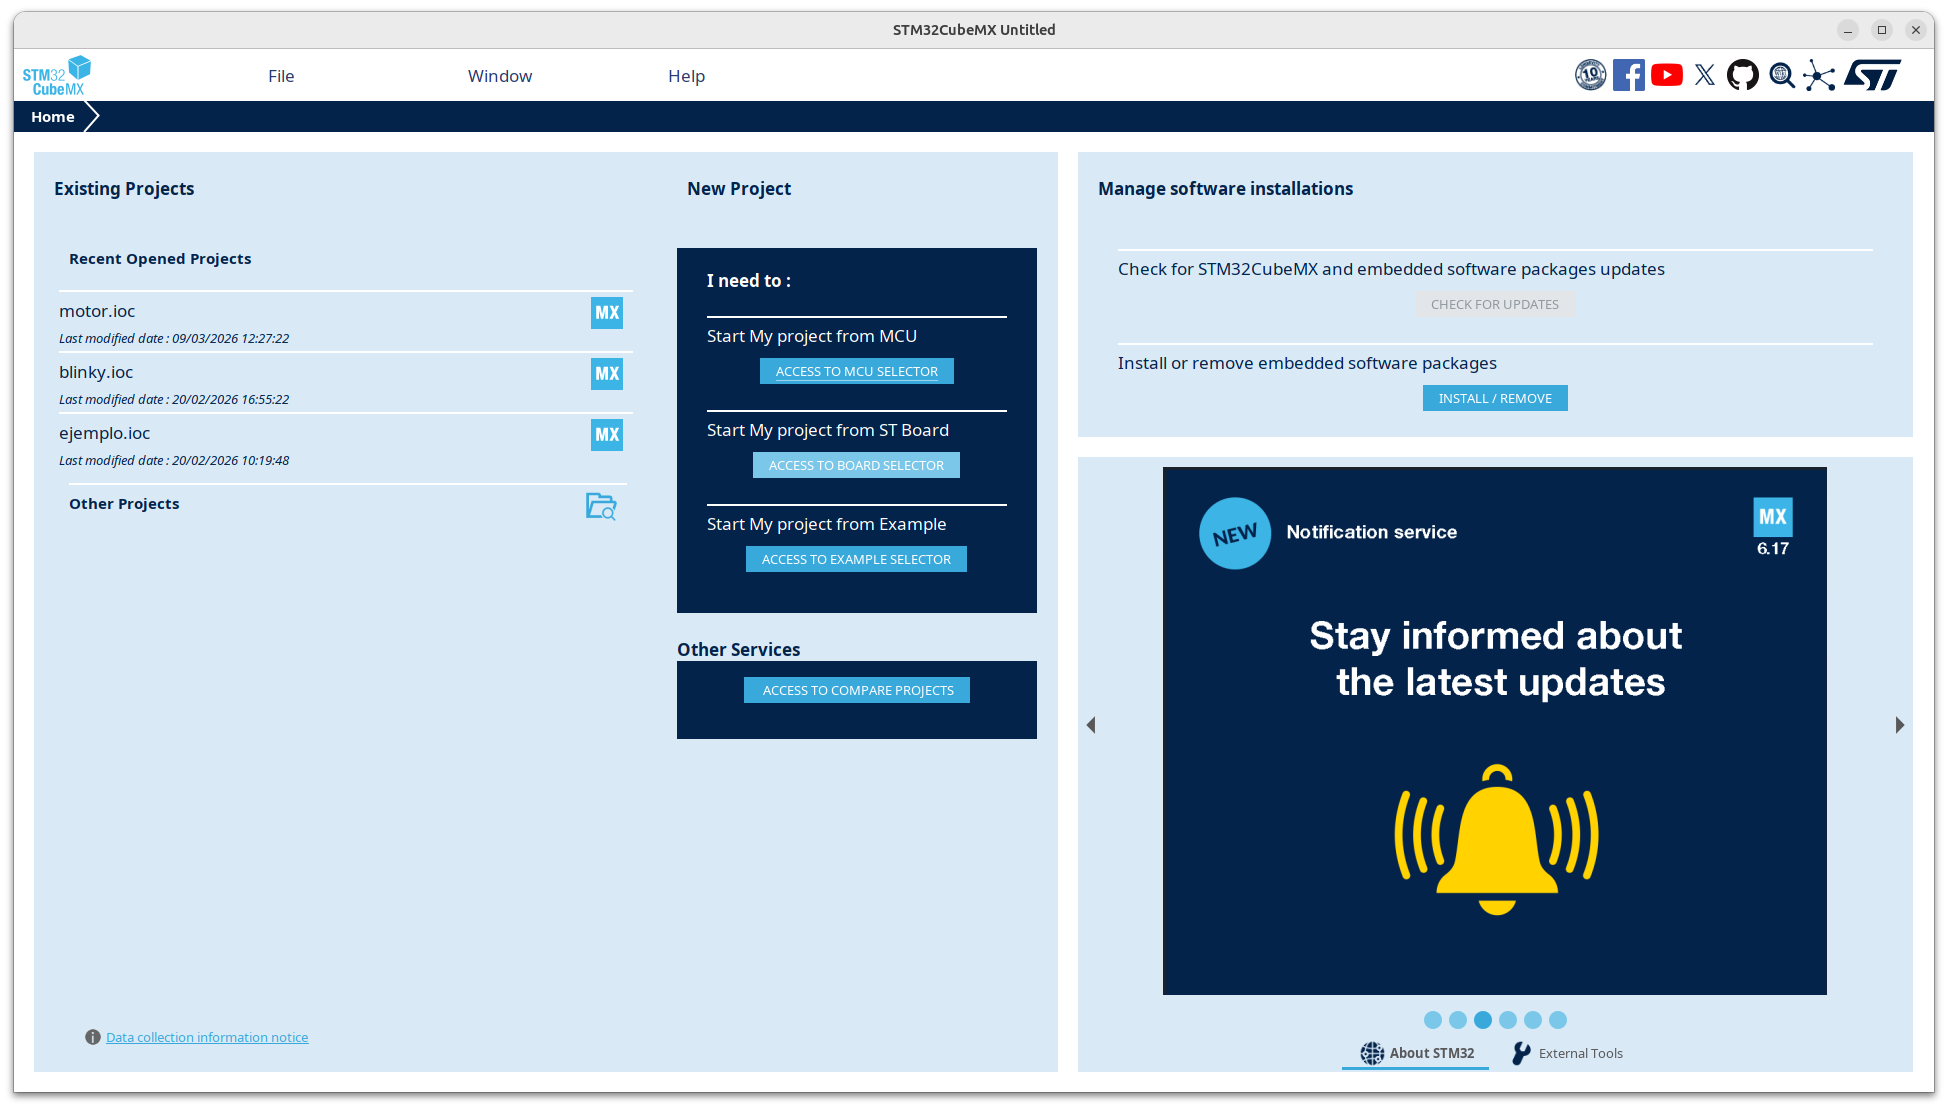
\includegraphics[width=0.45\linewidth]{MXstartup.png}
}
%no space
\hfill
\subfloat[Selección de la placa]{\label{fig:cdiagram}
\centering

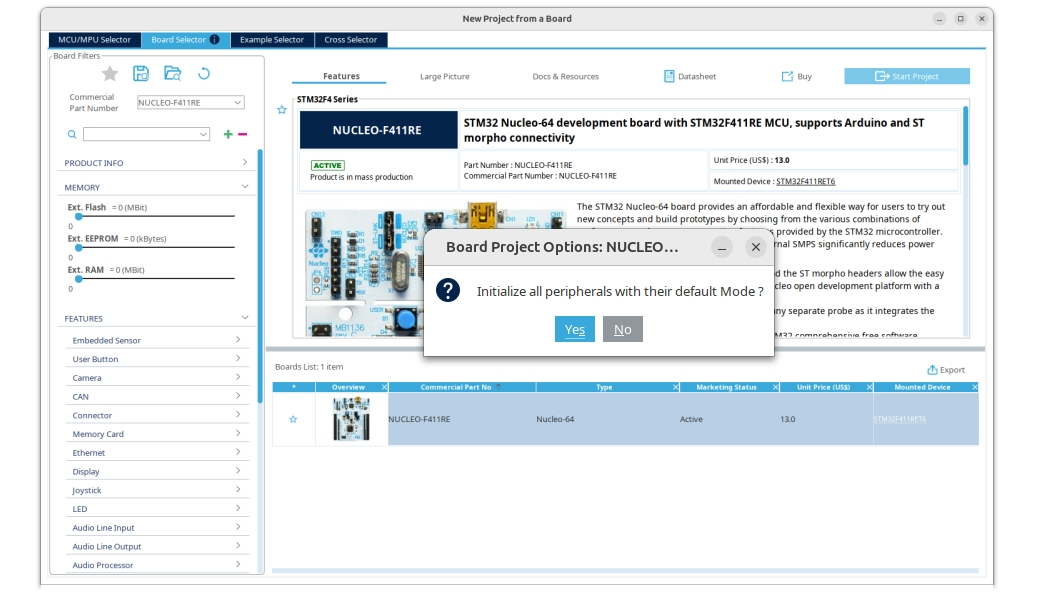
\includegraphics[width=0.45\linewidth]{Seleccionplaca.jpg}
}
\hfill

\subfloat[Layout de la placa NUCLEO F411RE]{\label{fig:layoutp}
\centering

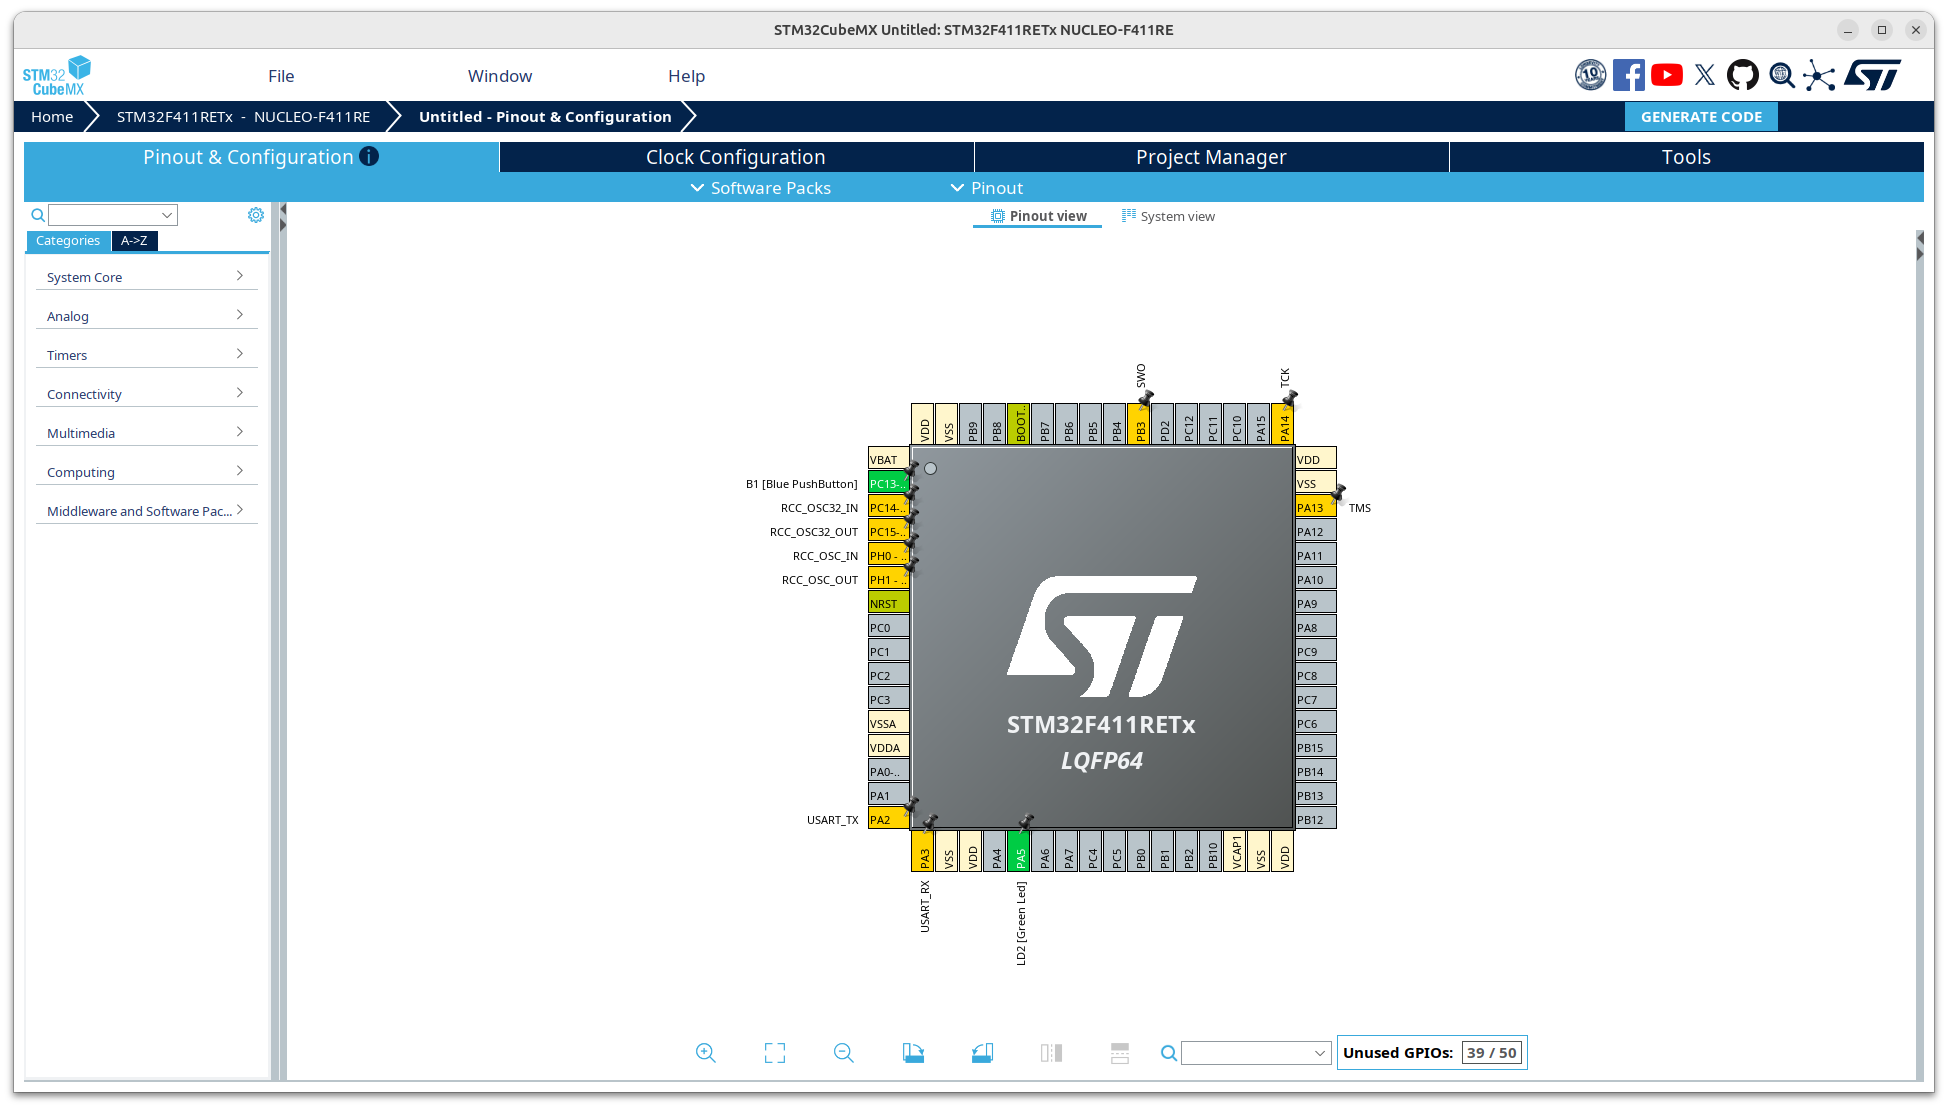
\includegraphics[width=0.45\linewidth]{layout_placa.png}
}
\subfloat[Debug a Serial wire y Reseteo del pin PB3]{\label{fig:PB3}
\centering

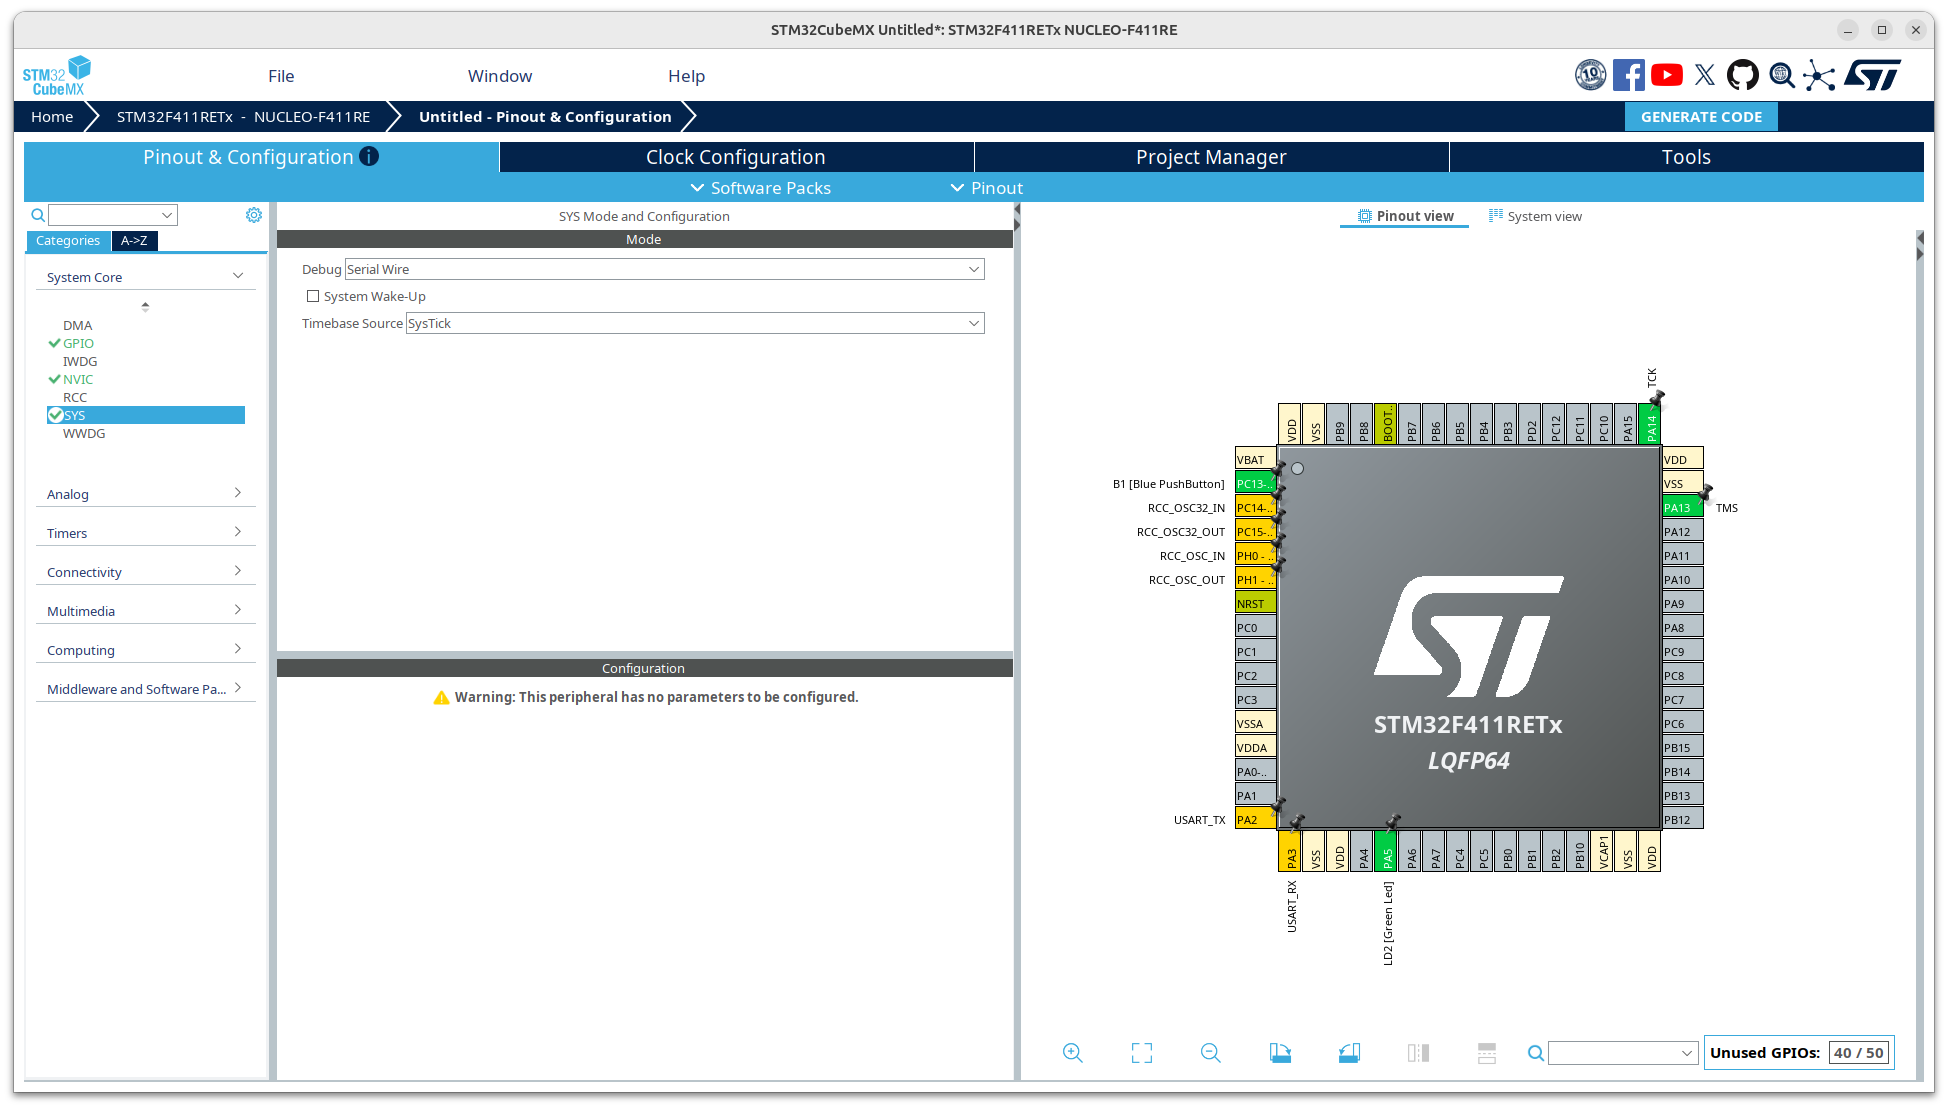
\includegraphics[width=0.45\linewidth]{pb3.png}
}
\hfill
\caption{Ventanas de inicio y selección de placa}
\label{fig:csetup}
\end{figure}

Vamos a establecer nuestras necesidades, de acuerdo con las posibilidades de la placa.
\section{Configuración del Reloj.}
Una de las características interesantes de la \emph{Black Pill} es su velocidad. Vamos a configurar el reloj de la placa para que trabaje a 100MHz, que es la máxima velocidad disponible.

Por defecto, la placa activa un reloj interno. Sin embargo, es mejor emplear el oscilador externo para general la señal de reloj, ya que nos da más precisión y nos va a permitir manejar con más velocidad y precisión las comunicaciones a través del puerto serie.

Para ello, volvemos a la categoría \texttt{System Core} y seleccionamos la entrada \texttt{RCC} (Reset and Clock Control). Buscamos la opción High Speed Clock (\texttt{HSE}). Cambiamos  "Disable" por \texttt{BYPASS Clock Source}. 
Hacemos esta elección porque en la placa, la señal de reloj la toma el microcontrolador directamente del programador (ST-Link). Los pines PH0 y PH1 aparecen ahora de color verde.

\paragraph{Configurar la frecuencia en el \emph{clock Tree}}
Buscamos ahora, en las pestañas de la parte superior, la que aparece marcada como \emph{Clock Configuration}. Se nos muestra un esquemático del árbol de configuración del reloj del microprocesador.
\begin{itemize}
\item  Nos aseguramos de que la casilla \texttt{Input Frequency} aparece el número 8 (8MHz, corresponde a la frecuencia de la señal de reloj envía al microcontrolador desde fuera).
\item En el multiplexor \texttt{PLL Source Mux}, marcamos la opción \texttt{HSE}.
\item En la casilla \texttt{HCLK (MHz)}, escribimos 100 (que es la velocidad máxima de la F411).
\item Pulsamos \texttt{Enter} y dejamos que CubeMX ajuste los divisores M,N,P,Q.
\end{itemize}

La figura \ref{reloj} muestra una imagen de la pestaña \emph{Clock Configuration}. Con el reloj ajustado a 100mHz.


\begin{figure}
	\centering
	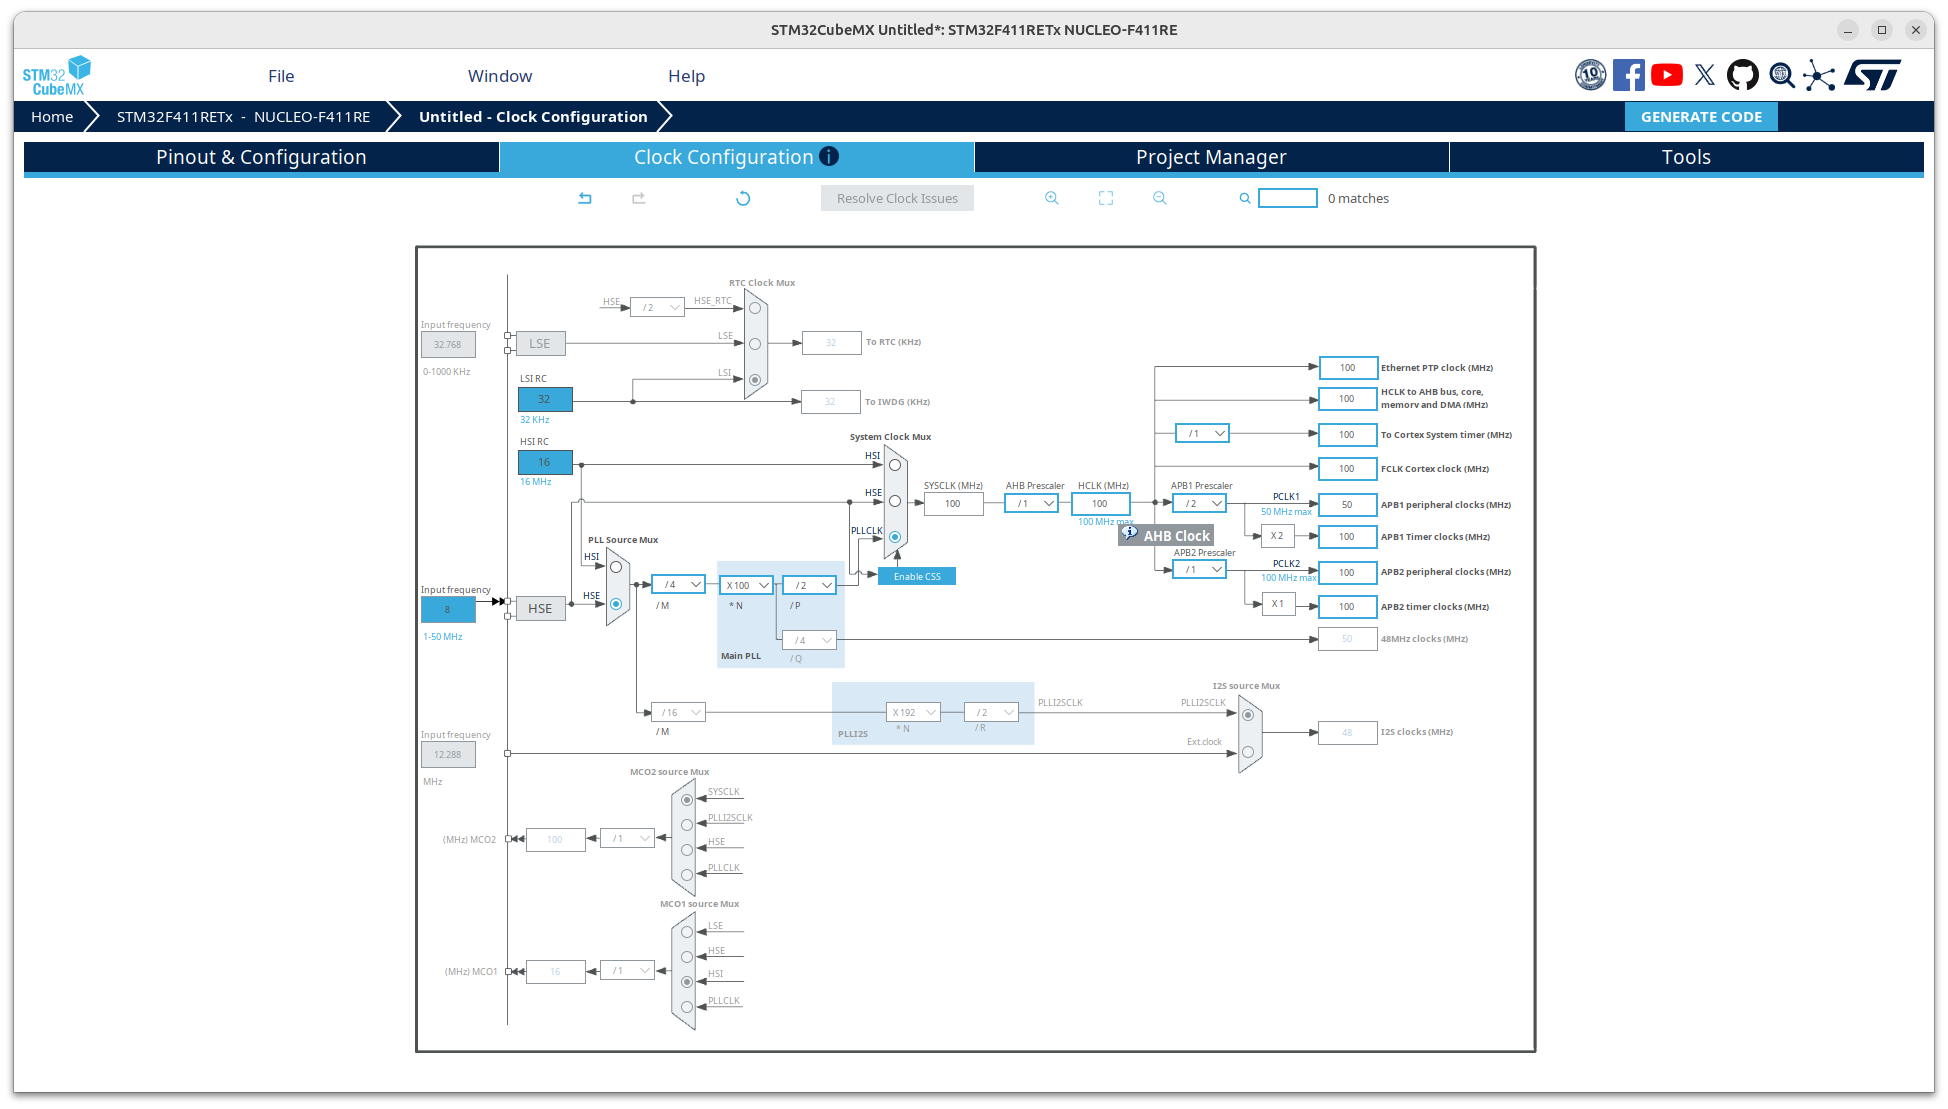
\includegraphics[width=\textwidth]{clock.png}
	\caption{Vista de la pestaña de configuración del reloj, con el reloj configurado a 100MHz.}
\label{reloj}
\end{figure}
\section{Configuración de un puerto serie (UART), a través del puerto USB de la placa.}
Para poder interactuar con el motor desde un ordenador, la que vamos a hacer es comunicarnos con la placa a través de un puerto serie.

El conector USB de la placa Núcleo F411RE que usaremos para programarla y darle energía ya tiene un conversor de puerto serie integrado (a través del chip ST-LINK que está en la parte superior de la placa). Físicamente, este chip está conectado a los pines PA2 (Transmisor - TX) y PA3 (Receptor - RX) de tu procesador, que corresponden al periférico USART2.

Para configurarlo, en la ventana del STM32CubeMX, volvemos a seleccionar la pestaña de la izquierda \emph{Pinout\&Cofiguration}. En el menú de la izquierda, desplegamos la categoría \emph{Connectivity} y hacemos clic en USART2.

En la ventana central (Mode), cambiamos \emph{Disable} por \emph{Asynchronous}. Los pines PA2 y PA3 cambian ahora a verde

Abajo, en la pestaña \emph{Parameter Settings}, la velocidad (Baud Rate) por defecto es 115200 Bits/s. Lo dejamos así, es la velocidad estándar. Simplemente habrá que tener en cuenta ese dato en la aplicación en Python que emplearemos en el ordenador para comunicarnos con la placa.

Además habilitamos una interrupción que permita a la placa recibir comandos desde el ordenador. Para ello, bajamos al panel \emph{Configuration}, seleccionamos la pestaña \texttt{NVIC Settings} y marcamos la casilla \emph{USART2 global interrupt}.

Por último vamos a habilitar dos canales de DMA (Acceso directo a memoria) tanto para la recepción como para el envío de datos. Esto es necesario ya que, como veremos más alante, vamos a configurar un timer (TIM4), para que fije  el ritmo al que actua el control del motor a 1KHz. Este ritmo es imposible de seguir por el puerto serie, no podemos por tanto emplearlo para enviar datos, o bloquearemos mientras envía el control del motor. De hecho, vamos a enviarlos a un ritmo de 10MHz. Los canales de DMA desacoplan la tarea de envío/recepción de la CPU, esta sencillamente \emph{delega} la tarea de copiar los datos desde/a memoria, al hardware del puerto serie y no se bloquea o interrumpe la recepción de datos.

Para habilitar el uso de DMA por parte del USART lo que hacemos es, en \emph{configuración}, señalar la pestaña \emph{DMA settings}. 

A continuación, pulsamos el botón \emph{add} seleccionamos USART2\_TX. COn esto definimos el canal de DMA que va a usar el puerto YSART2 para sus envíos (TX). Completamos la cofiguración,

\begin{enumerate}
\item Direction:  Memory To Peripheral(de la RAM a la UART).

\item Priority: low
\item Mode: Normal. (Existe un modo Circular, pero como tu código procesa "paquete a paquete", el modo Normal encaja perfecto con tu lógica actual).

\item Increment Address: Peripheral desmarcado (es un solo registro fijo), Memory marcado (para que vaya rellenando tu estructura byte a byte).

\item Data Width: Byte / Byte.
\end{enumerate}

Para habilitar un canal de DMA para la recepción de datos, procedemos igual. Pulsamos el botón add y ahora seleccionamos USART2\_RX. La configuración es exáctamente la misma, salvo para la dirección (Direction) que ahora será: Peripheral To Memory (de la UART a la RAM) y la prioridad que ahora seleccionaremos: high.



\section{Configuración del resto de pines para el control del motor}
Reproducimos a continuación la tabla del capítulo 2 del guión de la práctica, en que se describen los pines que se emplearán para suministrar potencia al motor y leer las señales de los encoders.

\begin{table}[h]
	\centering
	\begin{tabular}{|l|l|c|p{7.5cm}|}
		\hline
		\textbf{Componente} & \textbf{Señal Motor/Driver} & \textbf{Pin STM32} & \textbf{Función del Periférico (STM32CubeMX)} \\ \hline
		\multirow{2}{*}{Encoder} 
		& Canal A (Fase A) & \textbf{PA0} & \texttt{TIM2\_CH1} (Modo Encoder) \\ \cline{2-4} 
		& Canal B (Fase B) & \textbf{PA1} & \texttt{TIM2\_CH2} (Modo Encoder) \\ \hline
		\multirow{4}{*}{Driver Potencia} 
		& PWM (Voltaje) & \textbf{PB4} & \texttt{TIM3\_CH1} (Generación PWM) \\ \cline{2-4} 
		& DIR (Sentido)   & \textbf{PB3} & \texttt{GPIO\_Output} (Salida Digital) \\ \cline{2-4} 
		&Habilitar p. H ENA & \textbf{PA10} & \texttt{GPIO\_Output} (Salida Digital) \\ \cline{2-4} 
		&Habilitar p. H ENB & \textbf{PA7} & \texttt{GPIO\_Output} (Salida Digital) \\
		\hline
	\end{tabular}
	\caption{Mapa de conexiones nativas entre el sistema electromecánico y la placa STM32 Nucleo.}
	\label{tab:pines}
\end{table}

Como se deduce de la tabla, la interacción con la planta se delega en gran medida al hardware:
\begin{itemize}
	\item \textbf{Lectura del Encoder (PA0 y PA1):}
A diferencia de sistemas más simples donde se programan interrupciones por software para contar los pulsos, aquí conectamos las señales en cuadratura a los canales 1 y 2 del \texttt{Timer 2}. Al configurarlo en \textit{Encoder Mode}, el hardware del STM32 detecta automáticamente el sentido de giro y actualiza el registro del contador (\texttt{CNT}). Nuestro software simplemente leerá este registro cuando lo necesite.

Para configurarlo adecuadamente, en el panel lateral izquierdo \texttt{Categories} de la pestaña \texttt{pinout \& configuration}, Seleccionamos la entrada \texttt{timers}. Elegimos el timer \texttt{TIM2}. Se abrirá un nuevo panel para configurarlo. En dicho panel buscamos la opción \texttt{Conbined Channels}, despleagamos el menú y seleccionamos \texttt{Encoder Mode} Automáticamente nos pondrá loas pines \texttt{PA0} y \texttt{PA1} en color verde y les asignará, respectivamente los canales \texttt{CH1} y \texttt{CH2} del timer 2.

	
	\item \textbf{Generación de PWM (PB4):} Se conecta al canal 1 del \texttt{Timer 3}. El microcontrolador generará la señal de control de potencia (\textit{Duty Cycle}) en este pin. basándose en el valor que calculemos en nuestro bucle de control y escribamos en su registro de comparación (\texttt{CCR1}).
Para configuralo,
\begin{enumerate}
\item En la vista del microcontrolador (el dibujo del chip), buscamos el pin \texttt{PB4}, hacemos clic sobre él y seleccionamos \texttt{TIM3\_CH1}. El pin se pondrá amarillo.
	\item En la lista de la izquierda, seleccionamos  \texttt{Timers -> TIM3}.
	\item En \texttt{Clock Source}, seleccionamos \texttt{Internal Clock}.
	\item En \texttt{Channel 1}, seleccionamos \texttt{PWM Generation CH1}.
	\item  Abajo, en Parameter Settings, ponemos

    \texttt{Prescaler: 0}

    \texttt{Counter Period (ARR): 1000 - 1} 
\end{enumerate}
Al fijar el valor del prescaler a cero. Estamos empleando directamente los pulsos de reloj para generar la señal de pwm. El oeriod de la señal viene definido directamente por el valor del counter periodo, La frecuencia del reloj de nuestro mucrocontrolador la hemos ajustado a 100MHz, luego el reloj genera un pulso cada 10ns, el counter cuenta 1000 mil pulsos para definir un ciclo entero de la señal de PWM $10ns\times 1000 = 10\mu s$. este es el periodo de nuestra señal. Para definir el duty cicle, es decir, la parte de ese periodo que tendrá un valor alto, tenemos una resolución de 1000, precisamente el valor de nuestro counter periodo es decir puedo incrementarlo en pasos de 10ns.

	\item \textbf{Señal de Dirección (PB3):} Se configura como una salida digital estándar (\texttt{GPIO Output}). Escribir un nivel lógico alto (1) hará girar el motor en un sentido, y un nivel bajo (0) en el sentido opuesto, invirtiendo la polaridad en el puente en H.
	Para configurarlo, es suficiente con hacer click sobre el pin y seleccionar \texttt{GPIO\_output}.
	
	\item \textbf{Habilitar ambos puentes en H (PA10, PA7)} Habilitamos los dos puentes en H para alimentar el motor a través de ambos puentes a la vez. Estos pines deben estar siempre a nivel lógico alto (1). Los configuramos de modo análogo al anterior: hacemos click sobre ellos y seleccionamos \texttt{GPIO\_output}.
	\item \textbf{Emplear el botón azul de usuario para invertir manualmente el sentido de giro.}
Realmente, esto no es necesario salvo para controlar el manual el sentido de giro. El botón azul de la placa está conectado al pin \texttt{C13}. Lo que vamos a hacer es asociarlo a una interrupción para que cada vez que se pulse, la placa cambie el valor del pin inmediatamente. Para ello, Hacemos click en el pin \texttt{C13} y seleccionamos \texttt{GPIO\_EXTI13}. Para Package pgfkeys Error: I do not know the key '/tikz/fit', to which you passed '(tim4) (update) (cnt) (txdma)', and I am going to ignore it. Perhaps you misspelled it.activar la interrupción,
\begin{enumerate}
	\item En la lista de la izquierda, vamos a \texttt{System Core -> NVIC.}
	\item Buscamos la línea que dice \texttt{EXTI line[15:10] interrupts} y marcamos la casilla \texttt{Enabled}.
\end{enumerate}

\end{itemize}

\section{Habilitar un timer para que lea periódicamente el número de pasos (Encoders) que ha avanzado el motor.} 
La lectura de encoders se lleva a cabo a muy alta velocidad. Esto dará robustez a los controladores que desarrollaremos en la práctica. Vamos a habilitar un tercer timer (\texttt{TIM4}) para que, genere una interrupción  a tiempo fijo y, de este modo decidir cuando actua la acción de control. 

\begin{enumerate}
	\item Volvemos de nuevo al panel de la izquierda y en  \texttt{Timers} seleccionamos \texttt{TIM4}. 
	\item En el panel que se despliega inmediatamente a su derecha marcamos la casilla \texttt{Internal Clock}
	\item Elegimos el ritmo a que llamamos a nuestra acción de control $0.001s$, es decir vamos a emplear para el control una frecuencia de $1KHz$. Para ajustar la frecuencia, empleamos la expresión,
	\begin{equation*}
		F_{\text{interrupción}} = \frac{F_{\text{reloj}}}{(\text{PSC}+1) \times (\text{ARR}+1)}.
	\end{equation*}
Hemos ajustado el reloj de nuestro microcontrolador a $100MHz$. Así que si ajustamos el PSC (Preescaler) a $100 -1 $, estaremos dividiendo la frecuencia del reloj entre 100. Si además ajustamos el ARR (Counter period) a $1000 - 1$, volvemos a dividir la frecuencia del reloj entre mil, de modo que la frecuencia de la interrupción quedará $1e8/1e2/1e3 = 1000 Hz$. 

Bajamos \texttt{configuration} y en la pestaña \texttt{Parameter Settings}. Buscamos la sección \texttt{Counter settings}. En \texttt{Preescaler} escribimos $100-1$ y en \texttt{Counter Period} $1000 -1$.

\item Por último, para activar la interrupción, en la pestaña \texttt{NVIC Settings} Marcamos la casilla \texttt{TIM4 Global interrupt}.
\end{enumerate}

\section{Instalar y activar CMSIS-DSP}
Por último, antes de generar nuestro proyecto, vamos a configurarlo para que use la librería CMSIS-DSP (Cortex Microcontroller Software Interface Standard - Digital Signal Processing).

Es una suite de librerías desarrollada directamente por ARM (los creadores de la arquitectura de tu STM32) y está diseñada específicamente para exprimir al máximo los procesadores Cortex-M.

 Incluye un amplio número de funciones: Basic math functions, Fast math functions, Complex math functions, Filtering functions, Matrix functions, Transform functions, Motor control functions, Statistical functions, Support functions, Interpolation functions, Support Vector Machine functions (SVM), Bayes classifier functions,Distance functions, Quaternion functions. 

En CMSIS-DSP, las rutinas está escrita usando instrucciones en ensamblador específicas de ARM (como multiplicaciones y acumulaciones en un solo ciclo de reloj - MAC) y usa la FPU (Unidad de Coma Flotante) por hardware.

En nuestro caso, las vamos a emplear para implementar un PID y para realizar operaciones matriciales que nos permitan emplear control por realimentación en variables de estado estimadas.

Para instalar las librerías CMSIS-DSP, seleccionamos en la barra de menú superior de la pestaña \texttt{Pinout \& configuration},la opción que Software Packs y hacemos clic en \texttt{Select Components}. Se abrirá una ventana nueva con una lista de librerías.
(Nota: Si es la primera vez que se abre, puede que tarde unos segundos en conectarse a los servidores de ST para descargar el catálogo).
\begin{enumerate}
	\item Desplegamos la pestaña \texttt{ARM.CMSIS}. Buscamos la fila que dice \texttt{\emph{CMSIS}DSP}.

\	\item En la columna de la derecha (llamada Selection), hacemos clic y cambiamos la opción a \texttt{Source}.

    \item Hacemos clic en OK para cerrar esa ventana. 
    \item Volvemos a la pantalla principal del CubeMX. En la columna de la izquierda, abajo del todo seleccionamos \texttt{Software Packs}.
    \item La desplegamos y hacemos clic en ARM.CMSIS.
    \item En el panel central, aparecerá la opción \texttt{CMSIS DSP}. Activamos su casilla. 
\end{enumerate}

\section{Definir CMake para la compilación y el enlazado y obtener el esqueleto del código del proyecto}
Por último, dado que vamos a utilizar las herramientas de Visualstudio Code para compilar nuestro código, debemos añadir a nuestro proyecto las instrucciones para hacerlo empleando \texttt{CMAKE}, ya que esta es en Visualstudio la opción por defecto.

Para ello, seleccionamos la pestaña \texttt{Project Manager}. en la sección \texttt{Project Name} damos un nombre al proyecto, por ejemplo "motor". En la sección \texttt{Toolchain / IDE}, cambiamos la opción a \texttt{CMake}.

Con esto, hemos completado la configuración de nuestro proyecto. Solo queda pulsar el botón \texttt{GENERATE CODE}, situado arriba a la derecha de la ventana principal de CubeMX, para que se generen los archivos del lo que podríamos llamar el esqueleto de nuestro código. Creará una nueva carpeta con el nombre del proyecto (motor) y varias subcarpetas con todo el código generado. En la siguiente sección examinaremos en más detalle este código. 

Toda la información de configuración del proyecto queda guardada en un archivo con el mismo nombre del proyecto y extensión \texttt{.ioc} (\texttt{motor.ioc}). Podemos modificar la configuración de nuestro proyecto, abriendo dicho fichero con el CubeMX. Recuperaremos todas las opciones que hemos ido seleccionando a lo largo de este capítulo y tendremos la opción de cambiarlas o añadir nuevas opciones. Cada vez que completemos una nueva configuración deberemos pulsar la opción \texttt{GENERATE CODE} para generar un nuevo fichero \texttt{.ioc} con los cambios.

A partir de ahora, para simplificar las explicaciones, nos referiremos siempre a nuestro proyecto y al directoria que contiene su código con el nombre de \emph{motor}.  

\input{cp4.tex}
% !TEX root = making_of.tex
\chapter{Programación en Python de un monitorizador.}
Una vez terminada la descripción del código empleado por el microcontrolador para controlar el motor, nos queda describir el programa para manejarlo desde el ordenador. (Se aconseja tener el código del programa abierto para seguir mejor estas notas.)

En este caso, tenemos un solo programa Motor.py; un script de Python standard. Cuando se ejecuta, el script abre una ventana que muestra un panel de control (\emph{Dashboard}), que permite al usuario interactual con el motor y monitorizar la posición y la velocidad del motor. La figura \ref{figdb} muestra una imagen del panel de control. Su uso se detalla en el guión de la práctica y no se repetira aquí.
\begin{figure}
    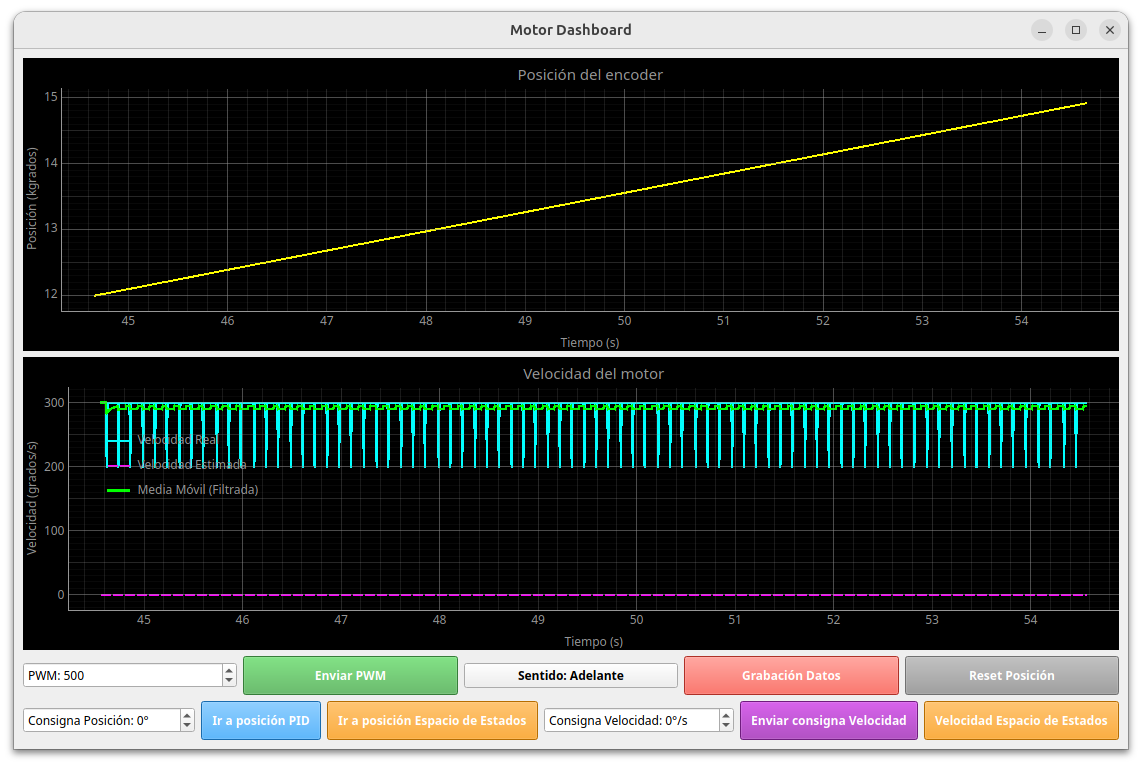
\includegraphics[width=\textwidth]{dashboard.png}
    \caption{Vista del panel de control desarrollado para interactual con el motor}
    \label{figdb}
\end{figure}

La ventana y los \emph{gadgets} se han desarrollado usando Qt, que es un \emph{framework} (conjunto de herramientas y bibliotecas) para desarrollar aplicaciones gráficas (interfaces de usuario, ventanas, botones, etc.) en C++, pero también está disponible para otros lenguajes como Python, Java, JavaScript, etc.
PyQt es la versión de Qt para Python, es decir, un binding (enlace) que permite usar todas las funcionalidades de Qt directamente desde código Python. Si nos fijamos en la cabecera del módulo \texttt{Motor.py}, podemos ver los módulos importados: serial, para manejar el puerto serie, struct para la gestión de los paquetes de datos, csv para general ficheros csv con los datos recibidos desde el microcontrolador, sys para gestionar comoandos del sistema operativo del ordenador, time para medir tiempos, collection para generar estrcturas de datos distintas de las estádar de python, datetime, para marcar fechas, pyqtgraph, QtCore, Qtwidgets para genera objetos gráficos con Qt y numpy para realizar operaciones matemáticas.

Despues de esto se definen dos variables globales, una de ellas es el nombre del puerto serie del ordenador donde se recibirán los datos procedentes del microcontrolador. Hay que recordar que en realidad, estos datos se entán recibiendo a través de un puerto USB que está emulando un puerto serie. El nombre asignado \texttt{PUERTO = '/dev/ttyACM0'} suele ser el típico asignado en Linux por defecto, peeeeero no es mala idea comprobar que efectivamente ese es el nonbre con el que el sistema operativo ha montado el puerto\footnote{para comprobarlo basta ir al directorio /dev y enchufar y desenchufar el cable USB, listando los archivos disponibles con ls deberá aparecer y desaparece ttyACM0 o el nombre del archivo donde el sistema lo ha montado}.

La segunda variable es la velocidad de transmisión del puerto que se fijado 115200 baudios que es la misma velocidad a la que se ha configurado el puerto serie en el microcontrolador.

El siguiente paso, es crear una clase, llamada \texttt{MotorDashboard} que contiene dentro todos los elemntos y funciones necesarios para levantar la ventana del panel de control.

Por último, si se ejecuta directamente Motor.py, se genera objeto tipo MotorDashboard, llamando al constructor de la clase, y se abre en el ordenador la ventana del panel de control \texttt{dashboar.show()}, lista para que el usuario la emplee. Cuando el usuario cierra la ventana el ordenador termina la ejecución del código y libera la memoria \texttt{sys.exit(app.exec\_())}.

Veamos ahora despacio la clase MotorDashboard.

\section{MotorDashboard}
La clase MotorDashboard contiene todas las funciones necesarias para crear el panel de control con el que el usuario puede interactuar con el motor a través de la placa de control, monitorizar las salidas (posición angular del rotor y velocidad) y almacenar datos en archivos tipo csv.
En la definición se pasa como parámetro la clase Qtwidgets.QMainWindow, de modo que MotorDashboar heredará de ésta todos sus métodos y atributos. Esta clase, esta asociada a Qt y permite crear la ventana principal de la aplicación y emplear todas las funciones y atributos asociados a las ventanas de Qt. A continuación se detallan todas las funciones que implenta la clase.

\subsection{El constructor.} Lo primero que hace el constructor de la clase, es llamar al constructor de la clase superior QMainWindow, de este modo se crea la ventana principal del panel de control, Además empleando los métodos setWindowTitle y resize, Da título a la ventana creada y le asigna un tamaño por defecto.

El siguiente paso es configurar el puerto serie. Para ello trata de crear un objeto Serial con el nombre del puerto y la velocidad (baudios) definidos previamente. Si no es capaz de establecer la comunicación, se cierra la aplicación y se nos muestra un mensaje de error en el terminal.

A continuación, se van creando tanto las variables necesarias para manipular los datos recibidos como los \emph{gadgets} necesarios para generar órdenes:
\begin{enumerate}
    \item se construyen cuatro buffers circulares, empleando estructuras de datos tipo \texttt{deque} del módulo collections. Estas estructuras son particularmente adecuadas por el método empleado para actualizar su contenido, Se crean buffers de 1000 datos uno para guardar los tiempos, otro para las posiciones medidas por el encoder, otro para las velocidades calculadas por el microcontrolador y un último buffer para la velocidad estimada por el observador.

    \item Se añaden variables para guardar los datos registrados en un archivo CSV.
    \item Se Configura la interfaz gráfica del panel de control. Se crea un panel principal \texttt{main\_widget = QtWidgets()}. Lo centra en la ventana de la aplicación \texttt{self.setCentralWidget(main\_widget)}. Se define una regla de ordenación vertical para los elementos que formen parte del panel central, de modo que se van apilando uno debajo del otro según se van creando \texttt{layout = QtWidgets.QVBoxLayout(main\_widget)}
    \item Se añade un gráfico, justo debajo del anterior, para representar la posición angular del motor leída por los encoders.
    \item Se añade debajo un gráfico en el que se van a representar, la velocidad calculada, la velocidad filtrada con el filtro de media móvil y la velocidad estimada 
    \item Se añade una primera fila de \emph{gadgets}, relacionados con el control manual del motor. Se decriben a continuación de izquierda a derecha; ver figura \ref{figdb}.
    \item \begin{enumerate}
        \item \texttt{spin} Es un \emph{spinbox}, es decir una caja en la que se puede escribir directamente un valor, o cambiar el valor mostrado empleando una flecha hacia arriba y una flecha hacia abajo. Permite seleccionar un valor de PWM entre 0 y 999, para definir manualmente el voltaje que se suministrará al motor. = corresponde a 0 voltios y 999 a 12.
        \item \texttt{btn\_send} Es un botón que envía el valor de PWM preseleccionado a la placa de control a través del puerto serie.
        \item \texttt{btn\_dir} Es un botón que permite alternar el sentido de giro del motor. Por defecto, el sentido de giro que aparece al arrancar el motor es \emph{sentido adelante}. Se corresponde con el giro del motor en sentido antihorario. Al pulsar esté botón cambia el sentido de giro, y también el texto que aparece escrito sobre él. Indicando el sentido de giro actual del motor.
        \item \texttt{btn\_record} Este botón activa/desactiva la grabación de datos en un fichero CSV
        \item \texttt{btn\_cero} Es un botón de reset, que para el motor, lo pasa a control manual y pone a cero todas las variables.
    \end{enumerate}
    \item Se añade una segunda fila de \emph{gadgets} relacionados con el control del motor. Se describen de izquierda a derecha; ver figura \ref{figdb}
    \begin{enumerate}
        \item \texttt{spin\_pos} Es un \emph{spinbox} que permite fijar la consigna de posición para el motor. De este modo el motor se moverá  hasta alcanzar dicha posición y pararse. Se ha limitado el rango a $[-3600, 3600]$ grados. Es decir se pueden fijar posiciones de más menos 10 vueltas a partir del punto donde se defina el cero, bien por los grados (pasos de encóder) leídos desde que se puso en marcha, bien por la posición de cero marcada por un reset.
        \item \texttt{bnt\_pos} Este botón, está etiquetado como \emph{ir a posición PID}. Cuando se pulsa se activa el control de posición mediante el uso de un PID. El eje del motor gira hasta alcanzar la posición de consigna indicada en el \emph{consigna de posición}; Spinbox anterior.
        \item \texttt{bnt\_pos\_ss} Este botón está etiquetado como \emph{ir a posición espacio de estados}. Cuando se pulsa se activa el control de posición empleando realimentación de estados estimados. El motor se mueve hasta alcanzar el valor de consigna indicado en la \emph{consigna de posición}.
        \item \texttt{spin\_speed} Análogo al spinbox descrito más arriba, solo que ahora permite ajustar el valor de la velocidad del motor. Se ha fijado un rango de velocidades $[-2000 2000]$ grados/s, que correspodería aproximadamente a cinco vueltas y media por segundo.
        \item \texttt{btn\_speed} Cuando se pulsa el motor acelera o decelera hasta alcanzar la consigna de velocidad fijada en \emph{consigna de velocidad}, spinbox anterior.
        \item \texttt{btn\_speed\_ss} Análogo al anterior, solo que ahora el control de velocidad se lleva a cabo empleando realimentación de estados estimados.   
    \end{enumerate}
    \item El siguiente paso es definir los eventos de los botones creados, es decir, asociar al pulsado de cada botón la función que ejecuta. Estas funciones son parte del objeto que estamos describiendo, pero no forman parte del constructor. Las describiremos más adelante indicando en la descripción cuál de los \emph{gadgets} que acabamos de describir, la activa.
    \item El último paso del constructor es definir un temporizador \texttt{timer = QtCore.QTimer()}, que utilizaremos para leer periodicamente los datos que llegan por el puerto serie. Este timer llamará cada 10ms a la función \texttt{read\:serial}, que describimos a continuación.
\end{enumerate}

\subsection{\texttt{read\_serial}}
Esta función juega un papel central en el funcionamiento del panel de control. Su papel es leer la trama de 20 bytes enviada por el microcontrolador, e interpretar su contenido.

Hay que recordar que esta función es llamada por el timer que hemos creado en el constructor de \texttt{MotorDashBoard} cada 10 ms.

Toda la función está contenida en un bucle while cuya condición de salida es una función del módulo serial que comprueba cuantos bytes quedan todavía en el buffer de entrada del puerto serie sin procesar, \texttt{in\_waiting >=20} Si hay al menos un paquete (20 bytes) entonces el bucle crea una bariable \texttt{paquete} en la que lee de golpe los primeros 20 bytes disponibles y los guarda e una variable llamada \texttt{paquete}

En la siguiente línea se emplea una estructura \texttt{try/except} para examinar el contenido de paquete y procesarlo. El paso siguiente sería emplear el comando \texttt{struct.unpack('<iiiff', paquete)} Para 'desempaquetar paquete en las variables que debe contener: \texttt{id\_paquete, valor1, posicion, velocidad, velocidad\_est}, donde \texttt{'<iiiff'} es un parámetro de formato que especifica que la codificación de los datos es litleedian '<', que los primeros cuatro bytes representan un entero 'i' y lo mismo para los cuatro siguientes y los cuatro siguientes; mientras que el penúltimo y último grupo de cuatro bytes representan dos floats 'f'.


\subsection{\texttt{send\_pwm}}
\subsection{\texttt{send\_position\_setpoint}}
\subsection{\texttt{send\_speed\_setpoint}}
\subsection{\texttt{send\_speed\_ss}}
\subsection{\texttt{toggle\_direction}}
\subsection{\texttt{sync\_direction\_ui}}
\subsection{\texttt{toggle\_recording}}
\subsection{\texttt{save\_csv}}
\subsection{\texttt{closeEvent}}
\subsection{\texttt{set\_zero\_position}}


\end{document}